\documentclass[a4paper, 11pt]{article}

\usepackage[english]{babel}
\usepackage[margin=1in, paperwidth=8.5in, paperheight=11in]{geometry}
\usepackage{amsfonts}
\usepackage{amsmath}
\usepackage{csquotes}
\usepackage{graphicx}
\usepackage{ amssymb }
\usepackage{cite}

\begin{document}
\begin{titlepage}
\begin{center}
\vspace*{1cm}
\textbf{\Huge{Learning to Learn}}\\
\vspace{0.5cm}
\textbf{\Large{Using Deep Networks with Memory Capacity}}
       
\vspace{2cm}
\textbf{Dr. Hien V. Nguyen}
        
\textbf{Aryan Mobiny}
        
\vspace{1cm}        
Department of Electrical and Computer Engineering\\
University of Houston\\
Houston, TX

\vspace{5cm}
\textbf{Abstract}
\end{center}
        
The goal of the proposed work is to replace the hand-designed update rule of the standard optimization algorithms (such as gradient descent, Newton\textsc{\char13}s method, etc.) with a learned update rule. Our project will investigate computational methods that can effectively learn update rules given a family of functions. Most of the current optimization algorithms have hand-designed update rules that exploit structure of a specific problem at hand. They, however, do not work well for problems outside of their scope. For example, the deep learning community and the sparsity community use very different set of optimization algorithms. We hypothesize that casting the design of optimization algorithm as a learning problem, called learning to learn or meta-learning, will allow the algorithm to learn to exploit structure of new optimization problems in an automatic way. We model the optimizer by recurrent neural networks such as Long Short Term Memory (LSTM) network and Differential Neural Computer (DNC). The optimizer is learned by varying weights of these networks. The recurrent networks enable our algorithm to compute the update rule based on not only the input data, but also the complete history of past updates. Our project proposes a novel objective function where we maximize the expected convergence rate instead of the original cost functions. We will evaluate our algorithms by training complex deep networks on large-scale database such as ImageNet and Visual7W.

        
\end{titlepage}

\section{Introduction}
Phrases like \enquote{I have experience in ...}, \enquote{This is similar to ...} or \enquote{This is a typical case of ...} imply that the person making such statements learns the task at hand faster or more accurately than an inexperienced human. This learning enhancement results from solution regularities in a problem domain \cite{hochreiter2001learning}. In a conventional machine learning approach, the learning algorithm mostly does not take into account previous learning experiences despite the fact that methods similar to human reasoning are expected to yield better performance. The use of previous learning experiences in inductive reasoning is known as\enquote{knowledge transfer} \cite{caruana1995learning, ellis1965transfer}. Here, we focus on one of the most appealing topics in knowledge transfer research field: \enquote{\textit{meta-learning}} or \enquote{\textit{learning to learn}}.

\emph{Learning to learn} is an exciting new research direction in designing optimization algorithms that can change the way they \emph{generalize}. Given a family of tasks, an algorithm is said to learn to learn if its performance at each task improves with experience and with the number of tasks \cite{thrun2012learning}. Put differently, an ordinary learning algorithm whose performance doesn\textsc{\char13}t depend on the number of learning tasks, which hence would not benefit from the presence of other learning tasks, is not said learn to learn. For an algorithm to fit this definition, some kind of transfer must occur between multiple tasks that must have a positive impact on expected task-performance. Generally speaking, learning to learn or meta-learning refers to a scenario in which an agent learns at two levels, each associated with different time scales. Rapid learning occurs within a task, for example, when learning to accurately classify emph{within} a particular data set. This learning is guided by a slower learning where knowledge is accrued gradually \emph{across} tasks to captures the way that task structure varies across target domains \cite{santoro2016meta}.

\vspace{1.5cm}
\section{Methodology}

In machine learning, tasks can be expressed as the problem of optimizing a cost function $f(\theta)$ and the goal is to find parameters $\theta$ that minimizes the cost $(\theta^*=\text{argmin}_{\theta} \ f(\theta))$. Among all possible methods to be applied, gradient descent is the standard approach for differentiable functions, resulting in the following sequence of updates:
\begin{eqnarray}
\theta_{t+1}=\theta_{t}-\alpha_t(\nabla f(\theta_{t}))
\end{eqnarray}
\noindent
where $\nabla f(\theta_{t})$ denotes the gradient of the function. While there are various types of problems of interest in different research areas, much of the focus in optimization works is based around such hand-designed update rules which make it suitable only to the specific problem at hand. In other words, exploiting the structure of the problem of interest for designing the optimizer comes at the expense of potentially poor performance on problems outside of that scope. The process of designing an optimizer is time and labor intensive, and limited to a small number of knowledgeable scientists.

Our project aims to use meta-learning to invent a learning algorithm that will perform well on any class of functions. To achieve that goal, our algorithm must be able automatically exploit structure of given optimization problems. To this end, we propose to replace the hand-designed update rule of gradient descent with optimizer $g$ which can be learned. The resulting updates of the objective function $f$ is of the following form:
\begin{eqnarray}
\theta_{t+1}=\theta_{t}+g_t(\nabla f(\theta_{t}),\varphi)
\end{eqnarray}
\noindent
where $\varphi$ denotes the set of parameters of optimizer g. This notation enables us to cast the design of optimization algorithm as a learning problem so that the resulting optimizers are specialized to particular classes of functions\cite{andrychowicz2016learning}. 

In order to model the update rule $g$, we can rely on the ability of deep networks to generalize to new examples by learning interesting sub-structures. Specifically, it\textsc{\char13}s been proposed that recurrent neural networks (RNN) are quite suitable to model the update rule $g$. Having internal memory enables RNN to maintain its own states and learn dynamic update rules which integrate information from the history of gradients.

\begin{figure}[t]
	\centering
	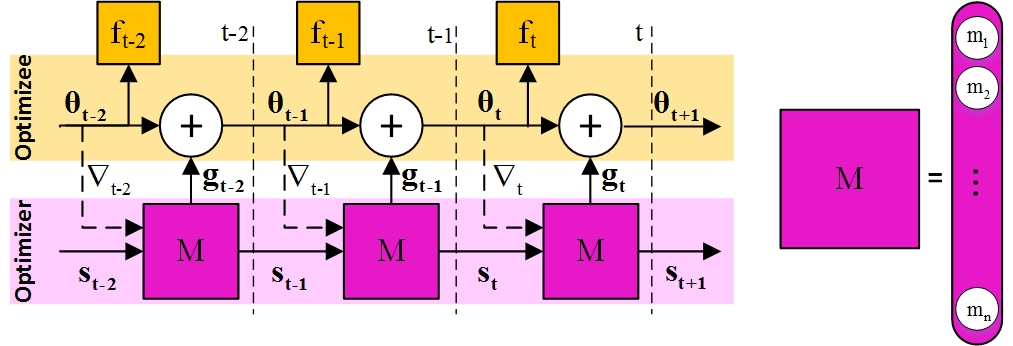
\includegraphics{Fig1.jpg}
	\caption{\textbf{Left:} Computational graph used for computing the gradient of the optimizer. \textbf{Right:} The optimizer block composed of replicated RNNs with shared parameters ($\varphi$), but separate hidden states}
\end{figure}

Computational graph of the proposed structure is shown in Figure 1. As noted earlier, we'll take the update steps $g_t$ to be the output of  recurrent neural networks (M) parametrized by $\varphi$, whose states we will denote explicitly with \textbf{s$_t$} and we will also use the notation $\nabla_t=\nabla_\theta f(\theta_t)$. 

Another aspect of high importance which is often overlooked has to do with the speed at which the algorithm converges.  In this sense, \enquote{rate of convergence}, the speed at which a convergent sequence approaches its limit, gives us a measure of the efficiency of the designed optimizer. We believe that while much of the focus in optimization works is on minimizing the cost function, inserting the rate of convergence in the problem of learning the optimizer and maximizing it is the key to achieve a suitable optimization algorithm. 
Given a sequence $x_1,\ x_2,\ \ldots,\ x_n$ , the rate of convergence of the sequence ($\alpha$) is defined as \cite{schatzman2002numerical}:
\begin{eqnarray}
\alpha\approx\frac{log{|(x_{n+1}-x_n)/(x_n-x_{n-1})|}}{log{|(x_n-x_{n-1})/(x_{n-1}-x_{n-2})|}}
\end{eqnarray}

Rewriting this equation by inserting the objective function results in
\begin{eqnarray}
\mathbb{E}[\alpha]=\mathbb{E}\left[\frac{log|[f(\theta_{n+1})-f(\theta_n)]/[f(\theta_n)-f(\theta_{n-1})]}{log|[f(\theta_n)-f(\theta_{n-1})]/[f(\theta_{n-1})-f(\theta_{n-2})]}\right]
\end{eqnarray}
\noindent
where the optimizee parameter $\theta$ can be considered as a function of the oprimizer parameters $\varphi$ and the objective function ($\theta(f,\varphi)).$


Next, other than inserting the convergence rate ($\alpha$), it's convenient to have an objective that depends on the entire trajectory of optimization, for some horizon T,

\begin{eqnarray}
\mathcal{L}(\varphi)=\mathbb{E}\left[\sum_{t=1}^{T}w_tf(\theta_t)-\lambda\alpha\right]\qquad \text{where}\qquad \theta_{t+1}&=&\theta_t+g_t,\\
\left[ \begin{matrix} g_t\\ s_{t+1} \end{matrix} \right]&=&\text{M}(\nabla_t,\textbf{s$_t$},\varphi).
\end{eqnarray}

Here $w_t\in\mathbb{R}$ are arbitrary weights associated with each time-step. In this objective function, fine-tunning the weight of the regularization term ($\lambda$) enables us to maximize the convergence rate at the same time with minimizing the optimizee function $f$ at each time-step. We can minimize the value of $\mathcal{L}(\varphi)$ using gradient descent on $\varphi$. The gradient $\partial\mathcal{L}(\varphi)/\partial\varphi$ can be computed by sampling a random function $f$ and applying backpropagation to the computational graph. We allow the gradients to flow along the solid edges in the graph, but gradients along the dashed edges are dropped. Ignoring gradients along the dashed edges amounts to making the assumption that the gradients of the optimizee do not depend on the optimizer parameters, i.e. $\partial\nabla_t/\partial\varphi=0$. This assumption allows us to avoid computing the second derivatives of $f$ \cite{andrychowicz2016learning}.

Examining the objective in (5) we see that the gradient of the first term ($\sum_{t=1}^{T}w_tf(\theta_t)$) is non-zero only for terms where $w_t\neq0$. If we use $w_t=1[t=T]$ to match the original problem, then gradients of trajectory prefixes are zero and only the final optimization step provides information for training the optimizer. This renders Backpropagation Through Time (BPTT) inefficient. This problem is solved by relaxing the objective such that $w_t>0$ at intermediate points along the trajectory. This changes the objective function, but allows us to train the optimizer on partial trajectories.


\begin{figure}[h]
	\centering
	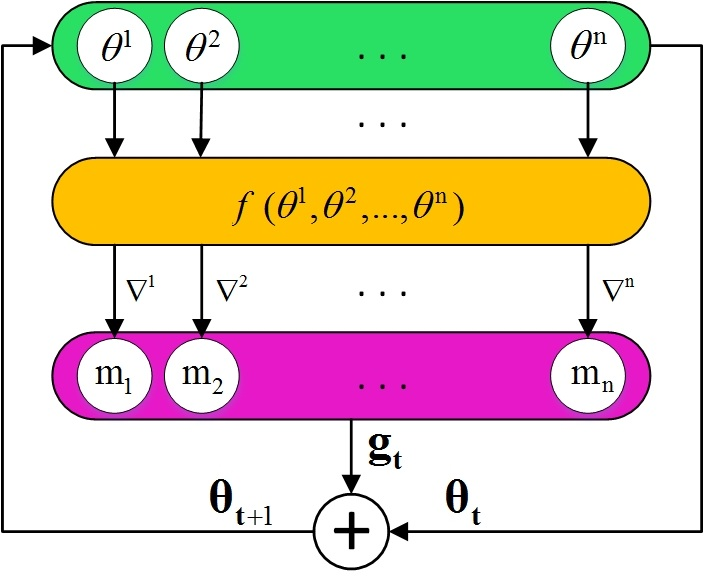
\includegraphics[scale=0.8]{Fig2.jpg}
	\caption{One step of an RNN optimizer}
\end{figure}

Figure 2 shows one step of updating the parameters using the proposed optimizer which implements the update rule for each coordinate using an RNN. As mentioned before, these RNNs have shared parameters, but separate hidden states. The network takes as input the optimizee gradient for a single coordinate as well as the previous hidden state and outputs the update for the corresponding optimizee parameter. The use of recurrence allows the optimizer to learn dynamic update rules which integrate information from the history of gradients,similar to momentum \cite{andrychowicz2016learning}. This is known to have many desirable properties in convex optimization (see e.g. \cite{nesterov1983method}) and in fact many recent learning procedures --such as ADAM-- use momentum in their updates.


 
To evaluate the performance of the proposed optimization algorithm, it needs to be implemented to several classes of experiments to see how well it can derive the learning algorithms from scratch. We will investigate whether our learned algorithm is able to outperform generic, hand-designed competitors on the problems for which they are trained, and also generalize well to new problems with similar structure. 

Our goal is to demonstrate this on various classes of problems, from optimizing simple convex functions to functions with sparsity and group sparsity constraints. Specifically, we plan to apply our method on the following regression task:
\begin{eqnarray}
\underset{\Gamma}{\operatorname{argmax}} \| \mathbf{Y} - \mathbf{D} \mathbf{\Gamma} \|^2 + \Omega (\mathbf{\Gamma})
\end{eqnarray}

\noindent
where $\mathbf{Y}$, $\mathbf{D}$, and $\mathbf{\Gamma}$ denote the input data, dictionary, and sparse coefficients, respectively. We will explore the optimization with different $\Omega (\mathbf{\Gamma})$ settings such as $\|\mathbf{\Gamma}\|_0$ and $\|\mathbf{\Gamma}\|_{1,2}$, corresponding to sparsity and group-sparsity constraints, respectively.

Recently, deep learning has become extremely active research topic due to its remarkable performance an array of important tasks, including image classification and natural language processing. However, many proposed deep networks are difficult to optimize. Heuristic techniques such as dropout and adding noise to the gradients are often used to avoid getting stuck at bad local minima. We will investigate our learned neural optimizer on training complex deep networks such as Differential Neural Computer and Neural Programmer. We will compare the performance of our optimizer with state-of-the-art methods used in deep learning community such as RMSprop, ADAM, and Nestrov\textsc{\char13}s accelerated gradient (NAG). Testing and evaluating the generalization of the learned optimizer to different architectures can be done for different applications and purposes, e.g., regression, image classification, image style transfer and synthesis, and by using various sources of data such as \textbf{MNIST} \cite{MNIST} (database of handwritten digits with tens of thousands examples) and \textbf{ImageNet} which is a large visual database, designed for use in visual object recognition research, with over fourteen million URLs of images that are hand annotated to indicate what objects are pictured \cite{ImageNet}. 

Even though Deep Neural Networks (DNN) can implement functions with higher complexity and so are capable of solving more complex problems than shallow ones, training deep nets has its own challenges. Even simple DNNs with only a few layers have thousands of parameters to be learned as well as hyper-parameters (such as initial parameter values, learning rates, etc.) that need to be tweaked by going through the whole cycle (training and evaluating the performance) few times. Given the large-scale data sets which are including millions of examples, this process could take hours, days, weeks and months depending on the size of the DNN model. Therefore, other than designing proper models, we face the battle to match the correct hardware devices for these training workloads. 

DNNs are structured in a very uniform manner such that millions of identical artificial neurons perform the same computation, i.e. matrix multiplication and convolution.   Therefore, the structure of a DNN fits quite well with the kinds of computation that a GPU with high memory bandwidth can efficiently perform, i.e. parallel computing or ability to do many things at once. Specifically, in the problem of designing and learning the proposed coordinatewise optimizers, using the Maxwell/Opuntia Clusters provided by the Center of Advanced Computing and Data Systems (CACDS) at the University of Houston would be a great help at both training  several coordinates in parallel and making inference about many different class of optimization problems with large-scale databases.

\pagebreak
\bibliographystyle{IEEEtran}
\bibliography{bibfile}


\end{document}
